\documentclass[pdftex,10pt,a4paper]{report}

	\usepackage[pdftex]{graphicx}
	\usepackage[textwidth = 200mm,margin = 15mm]{geometry}
	\usepackage{hyperref}

	\newcommand{\HRule}{\rule{\linewidth}{0.5mm}}

\begin{document}


\begin{titlepage}
\begin{center}

%\includegraphics[width=0.15\textwidth]{logo}~\\[1cm]

\textsc{\LARGE COS 314}\\[1.5cm]

\textsc{\large Neural Network}\\[0.5cm]

% Title
\HRule \\[0.4cm]
{ \huge \bfseries Project 3: Report  \\[0.4cm] }

\HRule \\[1.5cm]

% Author and supervisor
\noindent
\begin{minipage}{0.4\textwidth}
\begin{flushleft} \large
\emph{Author:}\\
u11013878 - Jaco \textsc{Bezuidenhout}\\




\end{flushleft}
\end{minipage}
\begin{minipage}{0.4\textwidth}
\begin{flushright} \large

\end{flushright}
\end{minipage}





\vfill

% Bottom of the page

{\large \today}

\end{center}
\end{titlepage}


\newpage

\pagenumbering{gobble}

\newpage
\pagenumbering{roman}

\tableofcontents 

\newpage
\pagenumbering{arabic}

\begingroup
\renewcommand{\cleardoublepage}{}
\renewcommand{\clearpage}{}
\chapter{Dataset}
\paragraph{I have used a web scraper to scrape data from 2 websites:}
\begin{itemize}
	\item{woes.co.za - Creative writing website for Afrikaans}
	\item{mibba.com - Creative writing in English}
\end{itemize}
I iterated through the pages and followed all the links to stories posted on the sites. From there I scraped the body of all the stories and used that to asynchronously calculate the frequencies of each of the 26 characters in the alphabet.\\ \\
On the Afrikaans website I have found that the url 'http://www.woes.co.za/bydrae/kortverhale/5' changes by 5 for every page. I then used 
	\begin{center}
		for (var page = 0; page < 600; page+=5) 
	\end{center}
to loop through all the pages to gather as many as possible data-sets to evaluate. The Afrikaans stories only counted to about 171 but it was enough to work with.\\ \\

On the English website the paging was easier on the page 'http://www.mibba.com/Stories/?page=1' and I could just use:
	\begin{center}
		for (var page = 0; page < 40; page++) 
	\end{center}
to page through all the pages. English stories was much easier to gather and here I ran through 535 stories.
\section{Number of chunks used}
\paragraph{I used different size chunks. All were greater than 300 characters. }	
\subsection{Afrikaans:}
	\begin{itemize}
		\item Training Dataset size: 81
		\item Generalization Dataset size: 90
	\end{itemize}	
\subsection{English:}	
	\begin{itemize}
		\item Training Dataset size: 425
		\item Generalization Dataset size: 110
	\end{itemize}	

\section{How frequencies were calculated}

When calculating the frequencies I used the callback function of the scraper to run through all the characters in the body of the stories. For every story I made an array of 26 values. With 0 as the default value. I first had to make the entire story lowercase and then I iterated through all the characters. If a (character's ordinal value (ascii value) minus 97) were between 0 and 26 (0 included and 26 not included), then I would increment the number stored in the array at the position of the (character's ordinal; value - 97). This array was appended to the language output file (afrikaans.txt or english.txt). Only the frequencies were stored in the file. This then acted as input data to the neural network.

\section{How special characters were handled}

After some research I decided to just simply ignore the special characters for it is not a clear trademark of the English or Afrikaans language. (If I looked at for instance Russian, then special characters would definitely not be ignored.) 

\section{Store format}
Example of a string in english.txt:
	\begin{center}
[0.07302904564315353, 0.025726141078838173, 0.02987551867219917, 0.04232365145228216, 0.1045643153526971, 0.017427385892116183, 0.02074688796680498, 0.04730290456431535, 0.0979253112033195, 0, 0.014937759336099586, 0.054771784232365145, 0.023236514522821577, 0.05975103734439834, 0.08132780082987552, 0.015767634854771784, 0, 0.030705394190871368, 0.06970954356846473, 0.07883817427385892, 0.038174273858921165, 0.01991701244813278, 0.027385892116182572, 0.0008298755186721991, 0.025726141078838173, 0],
	\end{center}

Each character's frequency are represented as the percentage of the character's occurrence in the entire text. The values were converted to the percentage values before stored into the file. This then allow the scraper to use various lengths of text to summarize the frequency of certain characters per language. 

\section{How the data was pre-processed}

The generalization set were made first. I tried to split the data as equally as possible (90 sets for Afrikaans and 110 sets for English). \\
The training set was not very equally split with 425 sets for English and 81 sets for Afrikaans.
				
\chapter{Experimentation}
\section{Changing Learning Rate}
\subsection{Settings}
\begin{itemize}
	\item Hidden layer neuron count: 10
	\item Momentum: 0.1
	\item Max Epochs 500
	\item Used the average of 30 iterations. 
	\item Learning rate: Changed by 0.1 every time.  
\end{itemize}
\subsection{Results}
\begin{center}
	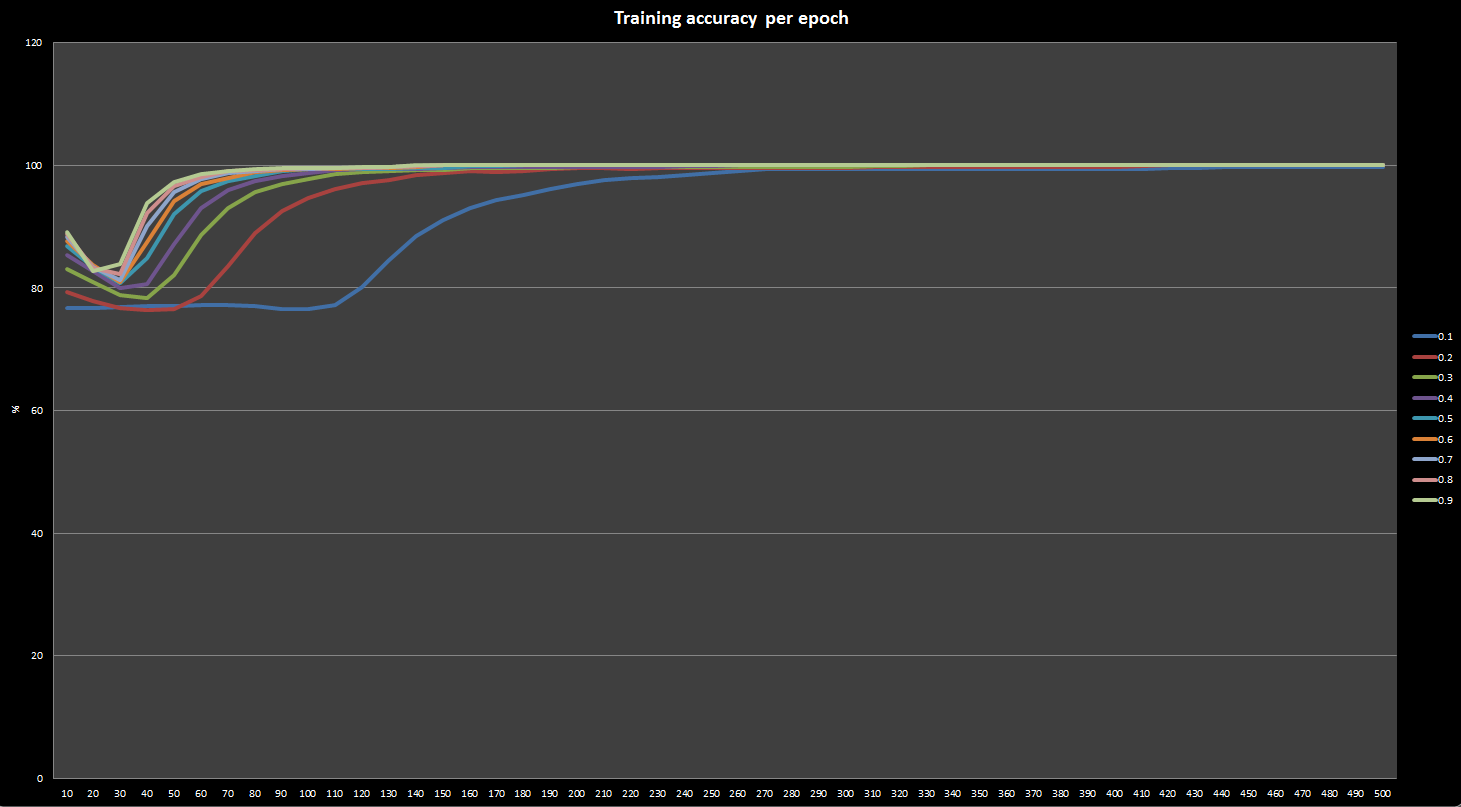
\includegraphics[scale=0.5]{charts/1_other}
\end{center}
\subsection{Conclusion}
In this experiment I have found that the smaller the learning rate. the longer it takes for the network to train to 100\%.\\
Here are the graph for this experiment containing the generalization accuracy as well. I have found that the generalization accuracy is directly dependent on the training accuracy.
\begin{center}
	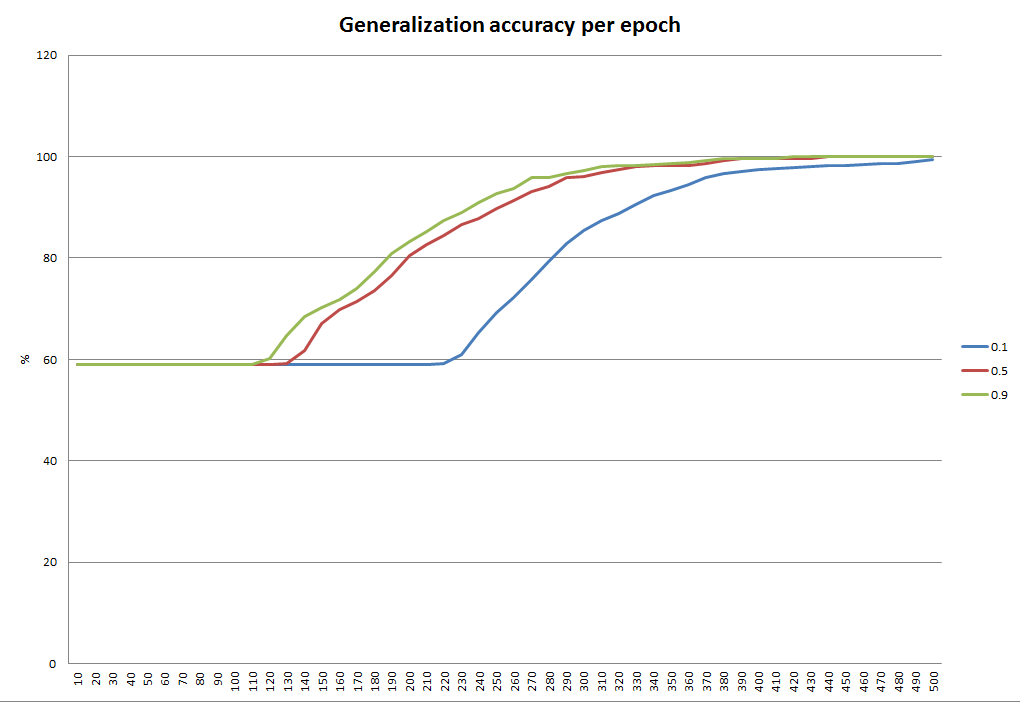
\includegraphics[scale=0.5]{charts/1_other_ag}
\end{center}
You can clearly see that the higher the learning rate, the faster the network train.

\section{Changing Momentum}
\subsection{Settings}
\begin{itemize}
	\item Hidden layer neuron count: 10
	\item Momentum: Changed by 0.1 every time.
	\item Max Epochs 500
	\item Used the average of 30 iterations. 
	\item Learning rate: 0.1  
\end{itemize}
\subsection{Results}
\begin{center}
	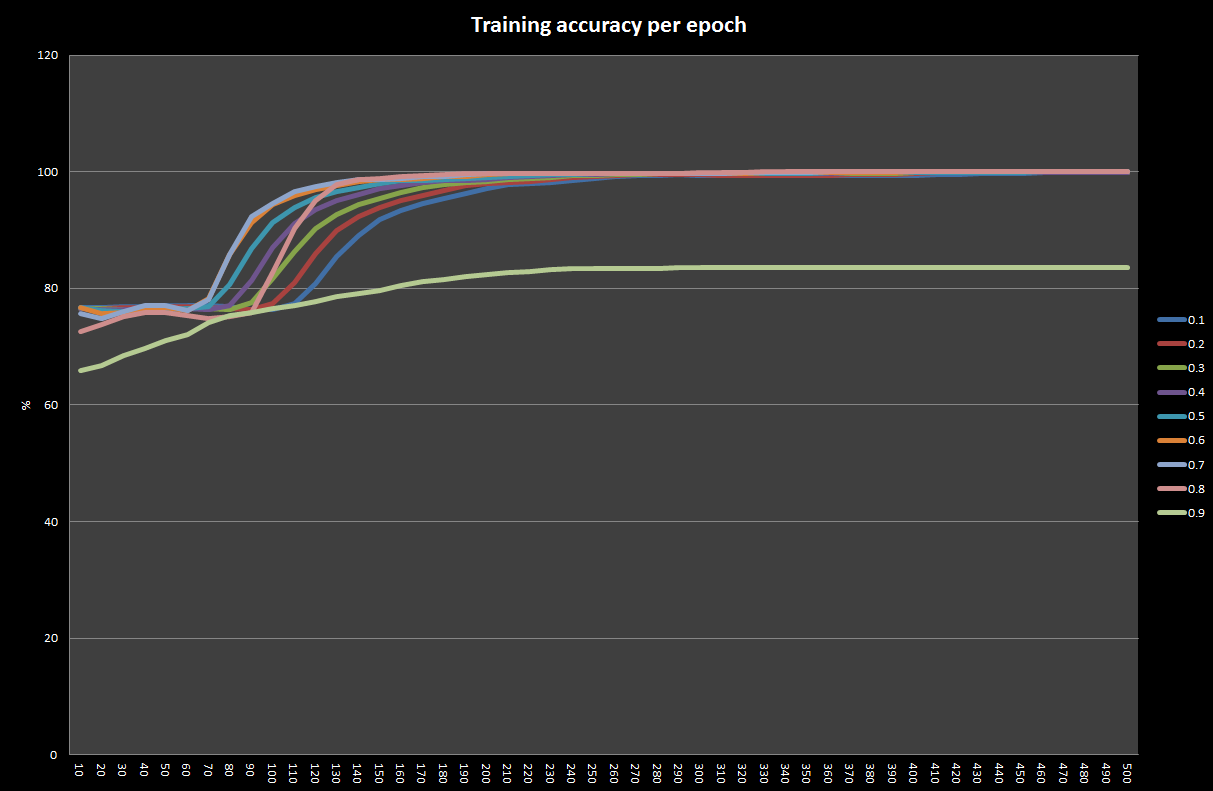
\includegraphics[scale=0.5]{charts/other_1}
\end{center}
\subsection{Conclusion}
In this experiment I have found that the smaller the momentum, the longer it takes for the network to train, but if the momentum is to high, then it has a negative effect on the entire training of the network. \\
Below are the graph for the generalization accuracy for this experiment for some momentum numbers.
\begin{center}
	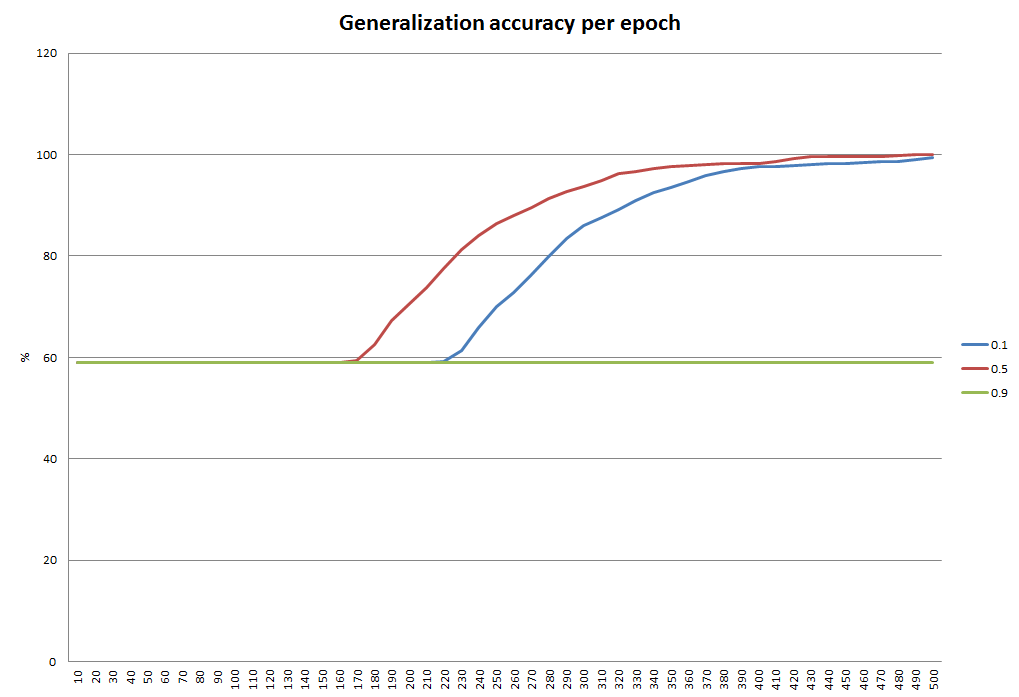
\includegraphics[scale=0.5]{charts/other_1_ag}
\end{center}
In this graph you can also see that a higher momentum train the network faster, but if it is too high, then the network do not train at all.
\section{Changing number of neurons in the hidden layer}
\subsection{Settings}
\begin{itemize}
	\item Hidden layer neuron count: Changed by 5 every time. Start 10. End 40.
	\item Momentum: 0.5
	\item Max Epochs 500
	\item Used the average of 30 iterations. 
	\item Learning rate: 0.5  
\end{itemize}
\subsection{Results}
\begin{center}
	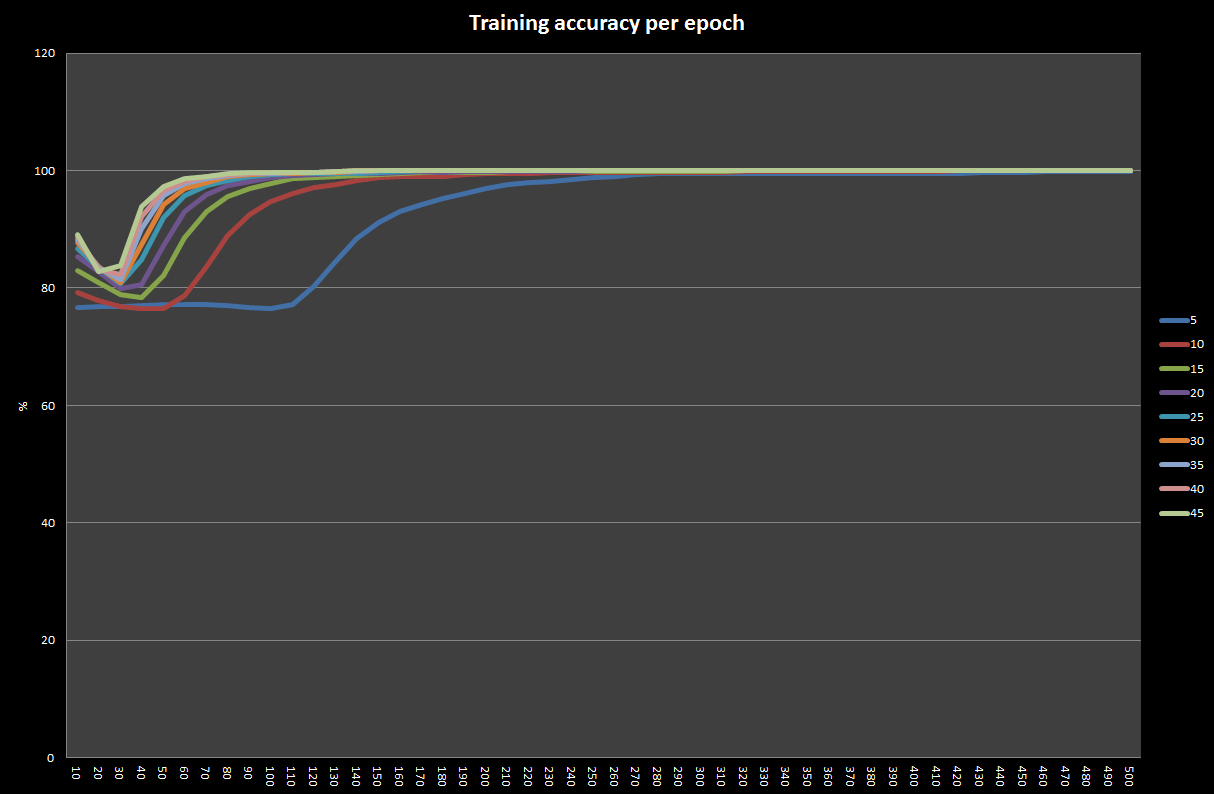
\includegraphics[scale=0.5]{charts/other}
\end{center}
\subsection{Conclusion}
In this experiment I have found that the higher the number of neurons in the hidden layer, the less epochs it takes for the network to train to 100\%.\\
Here are the graph for this experiment containing the generalization accuracy as well. When looking at the generalization accuracy you can see something strange.
\begin{center}
	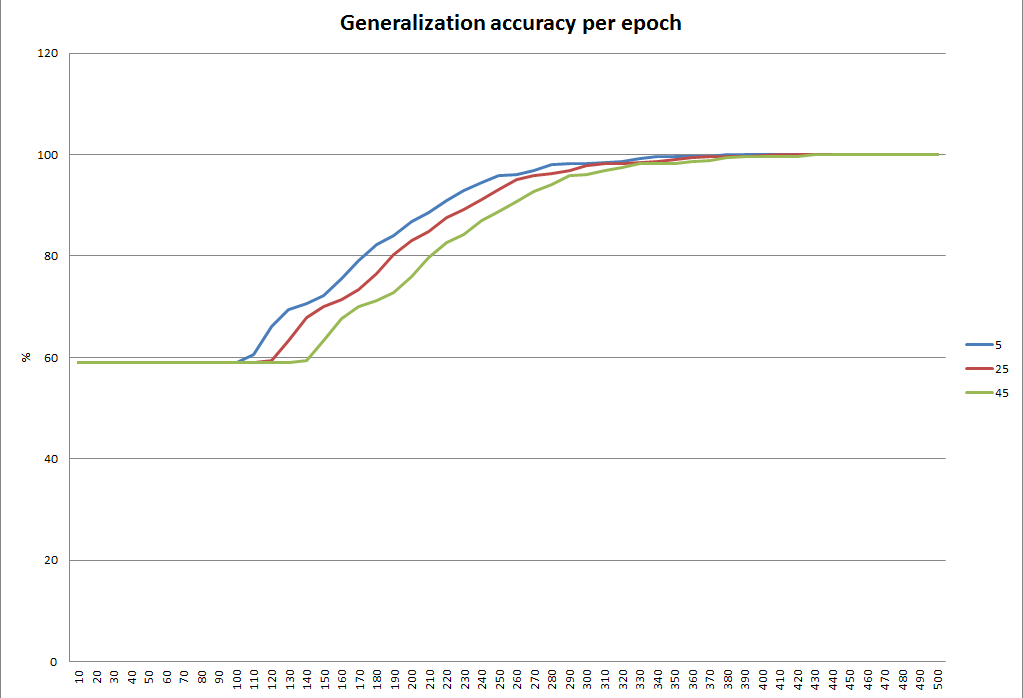
\includegraphics[scale=0.5]{charts/other_ag}
\end{center}
With this graph you can see that although the training accuracy are quicker to 100\% (previous graph), the generalization accuracy shows the complete opposite. Thus the more neurons in the hidden layer, the faster the network train but it is not the case when looking at how fast the generalization accuracy goes to 100\%.


\subsection{Main Conclusion}
In this experiment I have found that it is possible to use a neural network to learn how to classify Afrikaans and English. I have also found that the best setting, in my case, were:
\begin{itemize}
	\item Hidden layer neuron count: 10
	\item Momentum: 0.1
	\item Max Epochs 500 
	\item Learning rate: 0.9  
\end{itemize}

Here are a graph with some mixtures of the above data:\\
Line 1:
\begin{itemize}
	\item Hidden layer neuron count: 45
	\item Momentum: 0.9
	\item Max Epochs 500 
	\item Learning rate: 0.9  
\end{itemize}
Line 2:
\begin{itemize}
	\item Hidden layer neuron count: 15
	\item Momentum: 0.5
	\item Max Epochs 500 
	\item Learning rate: 0.5  
\end{itemize}
Line 3:
\begin{itemize}
	\item Hidden layer neuron count: 10
	\item Momentum: 0.1
	\item Max Epochs 500 
	\item Learning rate: 0.9  
\end{itemize}
\begin{center}
	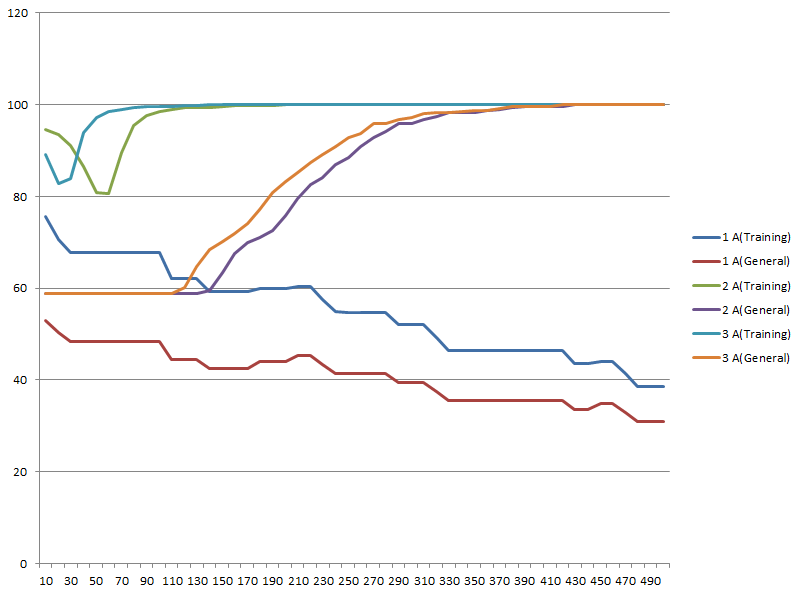
\includegraphics[scale=0.7]{charts/final}
\end{center}

I have also seen that the incorrect settings can either cause the system to execute very long before reaching 100\% accuracy (if learning rate or momentum are too small) or let the system diverge too much with every iteration (if the momentum value is to big).\\

The interesting part for me were the fact that the number of hidden neurons have a good effect on the training accuracy when higher, but it is in contrast with the generalization accuracy where less means more... 


\endgroup
	
\end{document}

